% !TEX TS-program = pdflatexmk
% !TEX encoding = UTF-8 Unicode

\documentclass[11pt,french]{article}

%Empagement courant (selon Hurtig : blancs tournants 2,1 2,625 3,15 3,675 en cm) 
%\usepackage[a4paper,twoside,textwidth=15.75cm,textheight=23.4cm,heightrounded]{geometry} 
\usepackage[a4paper,twoside,textwidth=15.75cm,textheight=25.5cm,heightrounded]{geometry} 
%\usepackage[a4paper,twoside,textheight=26cm,heightrounded]{geometry}

\usepackage[utf8]{inputenc}

%\documentclass[11pt,french]{article}
%\usepackage[utf8]{inputenc}
%\usepackage[letterpaper,body={6.0in,9.5in},vmarginratio=1:1]{geometry}

\usepackage{xcolor}

\usepackage[compact]{titlesec}

\newcommand{\MacTeX}{Mac\kern-.13em\TeX}
\newcommand{\BibTeX}{B\textsc{i\kern-.025em  b}\kern-.13em\TeX}
\newcommand{\TS}{\textsf{\TeX Shop}}
\newcommand{\latexmk}{\textsf{latexmk}}

\newcommand{\optkey}{\textsf{Opt}}
\newcommand{\ctlkey}{\textsf{Ctl}}
\newcommand{\cmdkey}{\textsf{Cmd}}
\newcommand{\esckey}{\textsf{Esc}}
\newcommand{\tabkey}{\textsf{Tab}}
\newcommand{\shiftkey}{\textsf{Shift}}

\newcommand{\mnu}[1]{\textsf{#1}}
\newcommand{\cmd}[1]{\textsf{#1}}
\newcommand{\To}{\,\(\to\)\,}
\newcommand{\Toto}{\,\(\leftrightarrow\)\,}


%Polices : Fourier for math | Utopia (scaled) for rm | Helvetica for ss | Latin Modern for tt
\usepackage[upright]{fourier} % math & rm
\usepackage[scaled=0.85]{berasans}
\usepackage[scaled=0.85]{beramono}
%\usepackage[scaled=0.875]{helvet} % ss
%\renewcommand{\ttdefault}{lmtt} %tt\usepackage{scrtime}

%Babel
\usepackage{babel}
\addto\captionsfrench{\def\tablename{\scshape Tableau}}
\frenchbsetup{ShowOptions,og=«,fg=»}
\usepackage{xfrac}
\usepackage[decimalsymbol=comma,unitsep=cdot,digitsep=thick,mode=text,sepfour=true,valuesep=thick]{siunitx}
\usepackage[np,autolanguage]{numprint}

%Caption, float, microtype
\usepackage{caption}
\usepackage{float}
\usepackage[final,babel]{microtype}

%HYPERREF
\usepackage[colorlinks=true,linkcolor=black,urlcolor=blue]{hyperref}
\begin{document}
\title{Utilisation de \latexmk\ avec \TS\thanks{Traduit par René Fritz le 16 mai 2013.}}
%\title{Quick Start Guide\\ to using\\ \texttt{latexmk} with \TS}
\author{Herbert Schulz\\\small\href{mailto:herbs2@mac.com}{herbs2@mac.com}}
\date{}


\maketitle
\thispagestyle{empty}

\section{Qu'est-ce que \latexmk\ ?}
%\section{What is \latexmk}?}

%Compiling a \cmd{tex} file containing cross-references, bibliographic references and/or indexes is a multi-pass process; i.e., you've got to run \cmd{(pdf/xe)latex} multiple times with possible intermediate runs of \cmd{bibtex} and/or \cmd{makeindex} until all references are resolved. The \latexmk\ \cmd{perl} program, rewritten and presently maintained by John Collins\footnote{The \latexmk\ web site is <\url{http://www.phys.psu.edu/~collins/software/latexmk-jcc/}>. You can get the latest version of \latexmk\ at <\url{http://www.phys.psu.edu/~collins/software/latexmk-jcc/versions.html}>. }, automates this multi-pass process. By default it first runs \cmd{(pdf/xe)latex} on a source file, determines file dependencies by examining the \cmd{log} and \cmd{aux} files produced by the run and then automatically runs \cmd{bibtex}\footnote{As of version 4.22 \latexmk\ will automatically choose between running \cmd{bibtex} or \cmd{biber} as required.} and/or \cmd{makeindex}, if needed, and the correct number of additional runs of \cmd{(pdf/xe)latex} to generate the bibliography, index and cross-references. Recent versions of \latexmk\ also work correctly with the \cmd{nomencl} package as well as the  \cmd{glossary} and \cmd{glossaries} packages and other packages that produce multiple bibliographies or indexes.


La compilation d'un fichier \cmd{tex} renfermant des références croisées, des références bibliographiques ou des index est un processus itératif, c.-à-d., que (\cmd{pdf/xe)latex} doit être exécuté plusieurs fois avec, éventuellement, des exécutions intermédiaires de \cmd{bibtex} ou \cmd{makeindex} jusqu'à ce que toutes les références soient résolues. Le programme \cmd{perl}, \latexmk\, réécrit et actuellement maintenu par John Collins\footnote{Le site web de \latexmk\ est <\url{http://www.phys.psu.edu/~collins/software/latexmk-jcc/}>.
Vous pouvez obtenir la dernière version de \latexmk\ sur <\url{http://www.phys.psu.edu/~collins/software/
latexmk-jcc/versions.html}>.}, automatise ce processus itératif. Par défaut, il compose le source d'abord avec (\cmd{pdf/xe)latex}, détermine les dépendances du fichier en examinant les journaux et fichiers auxiliaires produits par la compilation, et puis exécute automatiquement \cmd{bibtex}\footnote{Depuis la version 4.22 \latexmk\ choisira automatiquement de composer avec \cmd{bibtex} ou \cmd{biber} comme convenu.} ou \cmd{makeindex}, si nécessaire, et le nombre exact de compositions supplémentaires avec (\cmd{pdf/xe)latex} pour produire la bibliographie, l'index et les références croisées. Les versions récentes de \latexmk\ fonctionnent aussi correctement avec les extensions \cmd{nomencl}, \cmd{glossary} et \cmd{glossaries}, ainsi qu'avec d'autres extensions qui produisent des bibliographies multiples ou des index.


%\section{Quick Start!}
%
%This section will get you started quickly. Unless you are trying to customize the behavior of the supplied engines or want to use the more esoteric engines this really is all you need!

\section{Prise en main rapide}

Cette section vous permettra de démarrer rapidement. Sauf si vous essayez de personnaliser le comportement des moteurs fournis ou si vous voulez utiliser les moteurs les plus ésotériques, c'est vraiment tout ce qu'il vous faut !

%\subsection{Quick Install.}
%
%To activate the \latexmk\ \cmd{engine} files simply move all the files with extension \cmd{.engine} from \path{~/Library/TeXShop/Engines/Inactive/Latexmk/} two folder levels up, to \path{~/Library/TeXShop/Engines/}, and (re-)start \TS. (Note: \path{~/Library/} is the \cmd{Library} folder in your \cmd{HOME} folder.) When you click on the popup engine menu on the Source toolbar the newly enables engines names should appear; see Figure (\ref{fig:popupmenus}) to see how that menu changes. \textbf{Note: the engine names will \emph{not} appear in the \mnu{Typeset} Menu.}

\subsection{Installation}

Pour activer les fichiers \cmd{engine} de \latexmk\ il suffit de déplacer tous les fichiers de suffixe \cmd{.engine}  depuis \path{~/Library/TeXShop/Engines/Inactive/Latexmk/}, deux dossiers en amont, vers \path{~/Library/TeXShop/Engines/}, et de redémarrer \TS\ (\path{~/Library/} est le dossier \cmd{Library} de votre dossier \cmd{HOME}). Lorsque vous cliquez sur le menu déroulant des moteurs, dans la barre d'outils du source, les noms des nouveaux moteurs activés devraient apparaître ; consultez la \textsc{Fig.}\ref{figs:popupmenus} pour voir l'évolution du menu. \textbf{\textsc{Remarque}. -- Les noms des moteurs \emph{n'apparaissent pas} dans le menu \mnu{Composition}.}
 
%\subsection{Quick Use.}
%
%At the top of your Source file place the line
%\begin{verbatim}
%% !TEX TS-program = pdflatexmk
%\end{verbatim}
%to use the \cmd{pdflatexmk} engine which will use \cmd{pdflatex} to typeset your document. Substitute \cmd{latexmk} or \cmd{xelatexmk} for \cmd{pdflatexmk} to use \cmd{latex} or \cmd{xelatex} to typeset your Source. From then simply using \mnu{Typeset}\To\mnu{Typeset} (\cmd{Cmd-T}) will run through the complete process of fully typesetting your document.

\subsection{Utilisation}

Au début de votre fichier Source placez la ligne
\begin{verbatim}
% !TEX TS-program = pdflatexmk
\end{verbatim}
pour que le moteur \cmd{pdflatexmk} utilise \cmd{pdflatex} pour composer votre document. Pour utiliser \cmd{latex} ou \cmd{xelatex} pour composer votre source, remplacez \cmd{pdflatexmk} par \cmd{latexmk} ou \cmd{xelatexmk}. Dès lors, il suffit simplement d'utiliser \mnu{Composition}\To\mnu{Composer} (\cmd{Cmd-T}) pour que le processus complet se déroule jusqu'à l'entière mise en page de votre document. 

%\begin{figure}
%\centering
%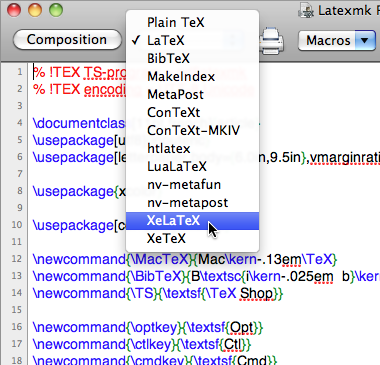
\includegraphics[width=2in]{figs/avant}\qquad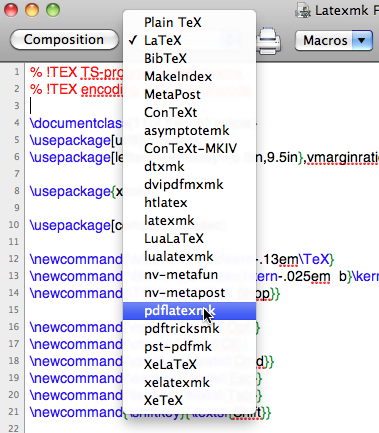
\includegraphics[width=2in]{figs/apres}
%%\caption{Default and updated versions of the engine pop-up menu after installing the \latexmk\ engines.\label{figs:popupmenus}}
%\caption{Évolution du menu des moteurs après l'installation des moteurs \latexmk.\label{figs:popupmenus}}
%\end{figure}

%\section{What is here?}
%
%There is a set of ten \cmd{engine} files to be placed in \path{~/Library/TeXShop/Engines/}. There is a \cmd{tslatexmk} folder already placed in \path{~/Library/TeXShop/bin/}. The files in that folder consist of the \cmd{latexmk} program, ten basic initialization (\cmd{rc}) files used by the ten \cmd{engine} files, a common file for personal settings (\cmd{latexmkrcDONTedit}) and two shell scripts used for \cmd{pdftricks} and \cmd{pst-pdf} figure processing. When any of the new engines is first run the \cmd{latexmkrcDONTedit} file will automatically be copied to \path{~/Library/TeXShop/bin/latexmkrcedit} if it doesn't already exist. You may copy the file there manually if you wish. \textbf{Any changes or additions to the configuration (e.g., new dependencies and rules) should be placed in the \cmd{laxtexmkrcedit} file. When \TS\ is updated the files in the \path{~/Library/TeXShop/bin/tslatexmk} may automatically get updated; don't edit them or your changes may get lost.}

\section{De quoi s'agit-il ?}

Il y a un ensemble de dix fichiers \cmd{engine} à placer dans \path{~/Library/TeXShop/Engines/}. Il y a un dossier \cmd{tslatexmk} déjà placé dans \path{~/Library/TeXShop/bin/}. Les fichiers de ce dossier comprennent le programme \cmd{latexmk}, dix fichiers d'initialisation de base (\cmd{rc}) utilisés par les dix fichiers \cmd{engine}, un fichier commun pour les réglages personnels (\cmd{latexmkrcDONTedit}) et deux scripts shell utilisés pour le traitement de la figure par \cmd{pdftricks} et \cmd{pst-pdf}. À la première exécution de l'un des nouveaux moteurs le fichier \cmd{latexmkrcDONTedit} sera automatiquement copié dans \path{~/Library/TeXShop/bin/latexmkrcedit} s'il  n'existe pas déjà. Vous pouvez copier le fichier manuellement à cet endroit si vous le souhaitez. \textbf{Tout les changements ou ajouts à la configuration (p. ex., de nouvelles dépendances et règles) doivent être placés dans le fichier \cmd{laxtexmkrcedit}. Lorsque \TS\ est mis à jour les fichiers dans le répertoire \path{~/Library/TeXShop/bin/tslatexmk} peuvent être automatiquement mis à jour ; ne les modifiez pas sous peine de perdre vos modifications}.

%\section{What is New with this Version}
%
%The engine files supplied with this version of latexmk for TeXShop now allow you to have a \cmd{platexmkrc} file, containing \cmd{latexmk} configuration information, in the same folder as the file you typeset (i.e., the root file for a distributed document). This can be useful if your project needs special configuration options for a certain task.
%
%E.g., you wish to use \cmd{texindy} instead of \cmd{makeindex} to process the \cmd{idx} file into a \cmd{ndx} file you might include a \cmd{platexmkrc} file in the same directory as the root file of a project with contents
%\begin{verbatim}
%$makeindex = "texindy %O -o %D %S";
%\end{verbatim}
%to use \cmd{texindy} rather than the default \cmd{makeindex}; make sure you end the file with a blank line. You could also add special options to the processing for a particular situation. Make sure you understand the syntax used by \cmd{latexmk} for customzing commands before playing with this feature.
%
%\textbf{One warning}: if you are going to use this feature understand that the \cmd{platexmkrc} file will be used for \emph{any} file in that folder that is typeset.

\section{Nouveauté dans cette version}

Les fichiers de moteur fournis avec cette version de \cmd{latexmk} pour \TS\ vous permettent désormais de disposer d'un fichier \cmd{platexmkrc}, contenant des informations de configuration pour \cmd{latexmk}, dans le dossier renfermant le fichier que vous composez (c.-à-d., le fichier racine du document distribué). Cela peut être utile si votre projet nécessite des options de configuration spécifiques à une tâche particulière.

P. ex., si vous souhaitez utiliser \cmd{texindy} au lieu de \cmd{makeindex} pour transformer le fichier \cmd{idx} en un fichier \cmd{ndx} vous pouvez inclure un fichier \cmd{platexmkrc}, dans le même répertoire que celui du fichier racine d'un projet, avec le contenu suivant,
\begin{verbatim}
$makeindex = "texindy %O -o %D %S";
\end{verbatim}
pour utiliser \cmd{texindy} plutôt que le \cmd{makeindex} par défaut ; veillez à ce que le fichier se termine bien par une ligne blanche. Vous pouvez également ajouter des options spéciales pour le traitement d'une situation particulière. Assurez-vous de bien comprendre la syntaxe utilisée par \cmd{latexmk} pour personnaliser les commandes avant d'exploiter cette fonction.

\textbf{Mise en garde} : si vous envisagez d'utiliser cette entité sachez que le fichier \cmd{platexmkrc} servira pour \emph{tous} les fichiers composés dans ce dossier.


%\section{Using \latexmk\ with \TS.}
%
%\textbf{NOTE: If you are updating to this version of \latexmk\ for \TS\ from a previous version you need only activate the engine files, as noted above, and restart \TS\ after installing the files.}
%
%There are ten \cmd{engine} files; two for running \cmd{latex} (one with a final run through \cmd{dvips} and \cmd{ps2pdf} [\cmd{latexmk.engine}] and one with a final run through \cmd{dvipdfmx} [\cmd{dvipdfmxmk.engine]}), two for using \cmd{pdflatex} [\cmd{pdflatexmk.engine} and \cmd{sepdflatexmk.engine}] (the second one for use when you need to use \cmd{-{}-shell-escape}), one for using \cmd{xelatex} [\cmd{xelatexmk.engine}], one for using \cmd{lualatex} [\cmd{lualatexmk.engine}], two for using the \cmd{pdftricks} or \cmd{pst-pdf} packages with \cmd{pdflatex} [\cmd{pdftricksmk.engine} or \cmd{pst-pdfmk.engine} respectively] and one for use with files that use the \cmd{asymptote} package [\cmd{asymptotemk.engine}]. The final engine is a very basic engine for typesetting \cmd{dtx} files for a package into the final documentation [\cmd{dtxmk.engine}]. The exact form of the commands and options used are in the corresponding \cmd{rc} file (e.g., \cmd{latexmkrc} for the \cmd{latexmk.engine}) in \path{~/Library/TeXShop/bin/tslatexmk/} and shouldn't be changed.
%
%You can use these \cmd{engine} files by using the drop down menu on the source tool bar or placing the line
%\begin{verbatim}
%% !TEX TS-program = pdflatexmk
%\end{verbatim}
%(for using \cmd{pdflatex}---similar lines for \cmd{latex} and \cmd{xelatex}, etc.) at the top of your document\footnote{For the dtxmk engine the line should be placed just below the initial ``\cmd{\% \textbackslash iffalse}'' line of the \cmd{dtx} file.}; then simply using \mnu{Typeset} (\cmd{\cmdkey-T}) will automatically run the proper \cmd{engine}. Note: these engines \emph{don't} appear under the \mnu{Typeset} Menu but only under the pop-up menu on the source toolbar. Figure (\ref{fig:popupmenus}) shows the default and updated pop-up menu after installing the \latexmk\ engine files.
%\begin{figure}
%\centering
%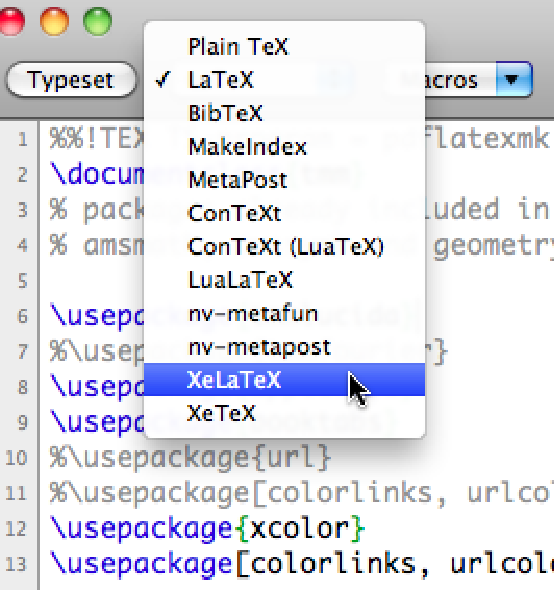
\includegraphics[width=2in]{figs/OriginalTypesetPopup}\qquad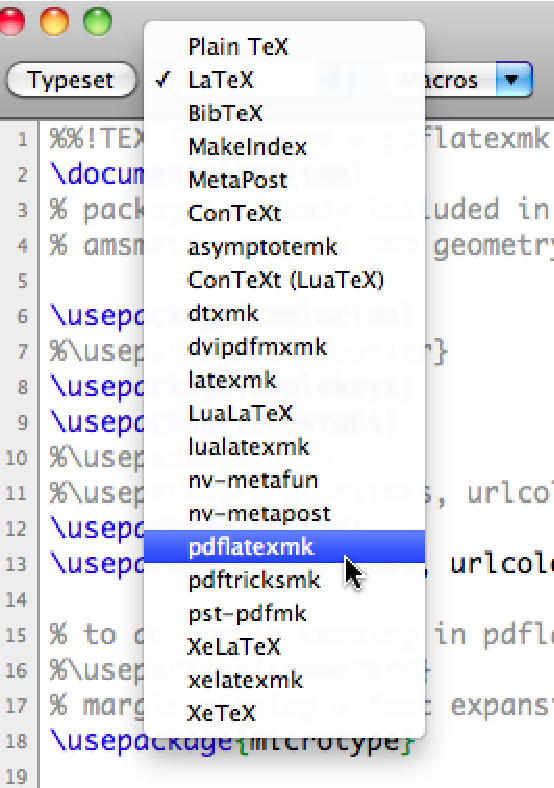
\includegraphics[width=2in]{figs/UpdatedTypesetPopup}
%\caption{Default and updated versions of the engine pop-up menu after installing the \latexmk\ engines.}\label{fig:popupmenus}
%\end{figure}
%
%Detailed information about using \latexmk\ with the \cmd{epstopdf}, \cmd{pdftricks} and \cmd{pst-pdf} packages is discussed later.
%
%I have only tested these engines with relatively trivial distributed documents (which include other files using \verb|\include| commands) but it appears that \latexmk\ deals with them properly. Note that when compiling a file with name \cmd{rootname.tex} a file with name \cmd{rootname.fdb\_latexmk}\footnote{The dependency file had extension \cmd{dep} in previous versions of \latexmk\ but didn't do a complete job of keeping track of those dependencies.} is created. This file contains the dependency information for the distributed document so making changes in an included file will force the recompile of the root document by \latexmk.


\section{Utilisation de \latexmk\ avec \TS}%%%

\noindent\textbf{\textsc{Remarque}. -- Si vous mettez à jour \latexmk\ à partir d'une ancienne version, il vous suffit d'activer les fichiers du moteur, comme indiqué ci-dessus, et de redémarrer \TS\ après l'installation des fichiers.}

Il y a dix fichiers \cmd{engine}, deux pour exécuter \cmd{latex} (un via \cmd{dvips} et \cmd{ps2pdf} [\cmd{latexmk.engine}] et un via \cmd{dvipdfmx} [\cmd{dvipdfmxmk.engine}]), deux pour exécuter \cmd{pdflatex} [\cmd{pdflatexmk.engine} et \cmd{sepdflatexmk.engine}] (le second à utiliser en cas de recours à \cmd{-{}-shell-escape}), un pour exécuter \cmd{xelatex} [\cmd{xelatexmk.engine}], un pour exécuter \cmd{lulatex} [\cmd{lulatexmk.engine}], deux pour utiliser les extensions \cmd{pdftricks} ou \cmd{pst-pdf} avec \cmd{pdflatex} [\cmd{pdftricksmk.engine} ou \cmd{pst-pdfmk.engine}, respectivement] et un pour des fichiers qui utilisent l'extension \cmd{asymptote} [\cmd{asymptotemk.engine}]. Enfin, un moteur très basique, sert à composer les fichiers \cmd{dtx} d'une extension vers son document final [\cmd{dtxmk.engine}]. La forme précise des commandes et options utilisées se trouve dans le fichier \cmd{rc} correspondant (p.~ex., \cmd{latexmkrc} pour \cmd{latexmk.engine}) situé dans \path{~/Library/TeXShop/bin/tslatexmk/} et ne devrait pas être changée.

Vous pouvez utiliser ces fichiers \cmd{engine} soit à partir du menu déroulant de la barre d'outils du source ou en plaçant la ligne
\begin{verbatim}
% !TEX TS-program = pdflatexmk
\end{verbatim}
(pour l'utilisation de \cmd{pdflatex} --- il y a des lignes similaires pour \cmd{latex} et \cmd{xelatex}, etc.) en haut de votre document\footnote{Pour le moteur \cmd{dtxmk} cette ligne doit être placée juste au-dessous de la ligne initiale « \cmd{\% \textbackslash iffalse} » du fichier \cmd{dtx}.} ; et il suffira d'utiliser \mnu{Composer} (\cmd{\cmdkey-T}) pour exécuter automatiquement le moteur requis. \textsc{Remarque}. -- Ces moteurs \emph{n'apparaissent pas} dans le menu \mnu{Composition} mais seulement dans le menu déroulant de la barre d'outil du source. La \textsc{Fig.}~\ref{figs:popupmenus} montre l'évolution de ce menu après l'installation des fichiers du moteur \latexmk.

\begin{figure}
\centering
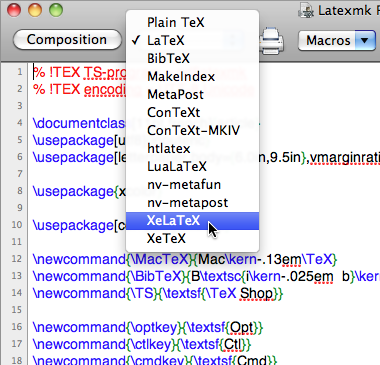
\includegraphics[width=2in]{figs/avant}\qquad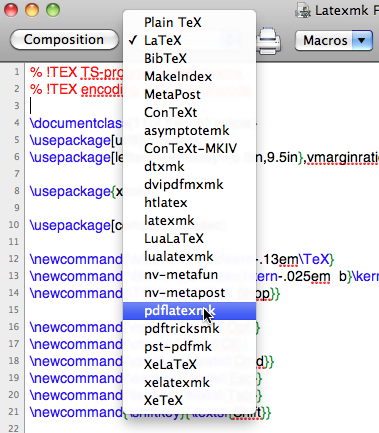
\includegraphics[width=2in]{figs/apres}
%\caption{Default and updated versions of the engine pop-up menu after installing the \latexmk\ engines.\label{figs:popupmenus}}
\caption{Évolution du menu des moteurs après l'installation des moteurs \latexmk.\label{figs:popupmenus}}
\end{figure}



L'utilisation détaillée de \latexmk\ avec les extensions \cmd{epstopdf}, \cmd{pdftricks} et \cmd{pst-pdf} est discutée ci-après.

Je n'ai testé ces moteurs qu'avec des documents distribués de façon relativement banale (qui incluent d'autres fichiers en utilisant des commandes \verb|\include|) mais il semble que \latexmk\ les traite correctement. Notez que lors de la compilation d'un fichier nommé \cmd{rootname.tex} un fichier nommé \cmd{rootname.fdb\_latexmk}\footnote{Dans la version précédente de \latexmk\ le fichier de dépendance possédait le suffixe \cmd{dep}, mais il ne remplissait pas complètement sa fonction de conservation des traces de ces dépendances.} est créé. Ce fichier contient l'information de dépendance du document distribué de sorte que la modification d'un fichier inclus forcera une nouvelle compilation du document maître \emph{(root)} par \latexmk.

%\subsection{Using the \cmd{epstopdf} package with \cmd{latexmk}.}%% < correction du format ligne 109

%\subsubsection{A word about \MacTeX\ 2009 \& 2010}
%
%% This is if embedded epstopdf in graphic(s/x) IS in MacTeX-2009
%There are two changes to the graphics sub-system that first appear in \MacTeX\ 2009:
%\begin{enumerate}
%%\item
%%The \cmd{graphic(s/x)} package now loads the \cmd{epstopdf} package when compiling with \cmd{pdflatex}. This is an attempt to make \cmd{eps} graphics inclusion under \cmd{pdflatex} a bit more transparent. (Note: This feature may not be present in the inital release of \MacTeX\ 2009.)
%\item
%The \cmd{epstopdf} package now defaults to using the \cmd{[update,append]} option. This has consequences if you don't use extensions when you include graphics files in your document.
%\item
%The default conversion is now \cmd{foo.eps}\To\cmd{foo-eps-converted-to.pdf}\footnote{This suffix can be customized.} to prevent any problems with overwriting a \cmd{foo.pdf} .
%\end{enumerate}
%The second of the changes to \cmd{epstopdf} leads to problems with \latexmk\ version 4.08 and earlier since the base file name changes. To make the latest \cmd{epstopdf} operate properly with latexmk version 4.08 and earlier I suggest creating an \cmd{epstopdf.cfg} file, to be placed in \path{~/Library/texmf/tex/latex/config} and containing the line
%\begin{verbatim}
%\epstopdfsetup{update,prepend,prefersuffix=false,suffix=}
%\end{verbatim}
%making \cmd{epstopdf} behave as before; the conversion becomes \cmd{foo.eps}\To\cmd{foo.pdf}. Using \latexmk\ version 4.10 or later requires no changes to \cmd{epstopdf} behavior but you may still do so if you wish to retain the pre-2009 behavior. You can find out the version number of the \latexmk\ program you are using by running the command
%\begin{verbatim}
%~/Library/TeXShop/bin/tslatexmk/latexmk -v
%\end{verbatim}
%in \cmd{Terminal}.
%
%Starting with \MacTeX\ 2010 the \cmd{graphic(x/s)} package will automatically load the \cmd{epstopdf} package if it detects that the file is being compiled using \cmd{pdftex} in \cmd{pdf} mode (normal for \cmd{pdflatex}). You no longer need to explicitly use the \cmd{epstopdf} package. Not only that but, if you haven't defined custom conversion and are only trying to convert \cmd{eps}\To\cmd{pdf} there isn't even a need to use the \cmd{-{}-shell-escape} flag: edit the \cmd{latexmkrcedit} file to eliminate it from all of the engines.


\subsection{Utilisation de l'extension \cmd{epstopdf} avec \latexmk}

\subsubsection{Un mot de \MacTeX\ 2009 \& 2010}

Dans \MacTeX\ 2009, il y a deux modifications au sous-système graphique :
\begin{enumerate}
\item 
L'extension \cmd{epstopdf} utilise maintenant, par défaut, l'option \cmd{[update,append]}. Cela a des répercussions si vous n'utilisez pas les suffixes lorsque vous incluez des fichiers graphiques dans votre document.
\item 
Pour prévenir tous problèmes d'écrasement d'un \cmd{toto.pdf}, la conversion par défaut est maintenant \cmd{toto.eps}\To\cmd{toto-eps-converted-to.pdf}\footnote{Ce suffixe peut être personnalisé.}.
\end{enumerate}

Ce second changement d'\cmd{epstopdf} engendre des problèmes avec les versions 4.08 et antérieures de \latexmk\ puisque le nom du fichier de base change. Pour que le dernier \cmd{epstopdf} fonctionne correctement avec les versions 4.08 et antérieures de \latexmk, je suggère de créer un fichier \cmd{epstopdf.cfg} qui sera placé dans \path{~/Library/texmf/tex/latex/config} et contiendra la ligne

\begin{verbatim}
\epstopdfsetup{update,prepend,prefersuffix=false,suffix=}
\end{verbatim}
afin qu'\cmd{epstopdf} se comporte comme avant ; la conversion devient \cmd{toto.eps}\To\cmd{toto.pdf}. À partir de la version 4.10, \latexmk\ ne nécessite aucune modification du comportement d'\cmd{epstopdf} mais vous pouvez encore le faire si vous souhaitez conserver le comportement d'avant 2009. Vous trouverez le numéro de la version du programme \latexmk\ que vous utilisez en exécutant la commande

\begin{verbatim}
~/Library/TeXShop/bin/tslatexmk/latexmk -v
\end{verbatim}
dans le \cmd{Terminal}

Dans le \MacTeX\ 2010, l'extension \cmd{graphic(x/s)} va automatiquement charger l'extension \cmd{epstopdf} si elle détecte que le fichier est compilé à l'aide \cmd{pdftex} en mode \cmd{pdf} (normal pour \cmd{pdflatex}). Vous n'avez plus besoin d'utiliser explicitement l'extension \cmd{epstopdf}. En outre, si vous n'avez pas défini de conversion personnalisée et essayez seulement de convertir \cmd{eps}\To\cmd{pdf} il n'est même pas nécessaire d'utiliser l'indicateur \cmd{-{}-shell-escape} : modifiez le fichier \cmd{latexmkrcedit} pour l'éliminer de l'ensemble des moteurs.

%\subsubsection{Working with \cmd{epstopdf}.}
%
%Versions of \cmd{epstopdf} from 1.5 on will automatically update a previously generated \cmd{pdf} file if the corresponding \cmd{eps} file is updated\footnote{Versions of \cmd{epstopdf} earlier than 1.5 never updated the \cmd{pdf} file once it existed.}. To let \latexmk\ ``know'' that it should allow runs of \cmd{pdflatex} if the corresponding \cmd{eps} file is updated the necessary \cmd{rc} files (the ones that run \cmd{pdflatex} rather than \cmd{latex}; \cmd{pdflatexmkrc}, \cmd{pdftricksmkrc}, \cmd{pst-pdfmkrc} and \cmd{asymptotemkrc}) contain a special dependency and rule
%\begin{verbatim}
%add_cus_dep('eps', 'pdf', 0, 'cus_dep_require_primary_run');
%\end{verbatim}
%which passes \latexmk\ the proper behavior.
%
%If you are using \cmd{epstopdf} 1.5 or later with earlier \TeX\ distributions you should invoke it using the \cmd{[update,prepend]} options. For versions of \cmd{epstopdf} earlier than 1.5 you should edit the \cmd{pdflatexmkrc}, \cmd{pdftrcksmkrc}, \cmd{pst-pdfmkrc} and \cmd{asymptotemkrc} files by commenting out the original dependency (place a \cmd{\#} before the line %% < pdftricksmkrc à corriger
%\begin{verbatim}
%add_cus_dep('eps', 'pdf', 0, 'cus_dep_require_primary_run');
%\end{verbatim}
%in that file) and uncommenting the new dependency (remove the \# from the start of the line
%\begin{verbatim}
%#add_cus_dep('eps', 'pdf', 0, 'cus_dep_delete_dest');
%\end{verbatim}
%in that same file). This will have \latexmk\ remove the \cmd{pdf} file before running \cmd{pdflatex} so \cmd{epstopdf} will recreate the \cmd{pdf} file. NOTE: These files may be automatically updated when \TS\ is updated and you may lose your changes!
%
%%You can use the same (default with this distribution) processing with \cmd{epstopdf} 1.5 and later, however the \cmd{epstopdf} package, version 1.5 and later can check for an updated \cmd{eps} file and then recreate the \cmd{pdf} file if the \cmd{[update,prepend]} package options are used.  The dependency checking by \latexmk\ is still important to let \latexmk\ ``know'' that an included \cmd{eps} file has changed but the deletion of the \cmd{pdf} image file is unnecessary.  The \cmd{pdflatexmkrc}, etc., support files for \latexmk\ 4.01 and later now contain a dependency and rule that will detect an updated \cmd{eps} file but let \cmd{epstopdf} do the conversion to \cmd{pdf}. By default this dependency is turned \emph{off} in \cmd{pdflatexmkrc}; to turn it on you should edit that file by commenting out the original dependency (place a \# before the line
%%\begin{verbatim}
%%add_cus_dep('eps', 'pdf', 0, 'cus_dep_delete_dest');
%%\end{verbatim}
%%in that file) and uncommenting the new dependency (remove the \# from the start of the line
%%\begin{verbatim}
%%#add_cus_dep('eps', 'pdf', 0, 'cus_dep_require_primary_run');
%%\end{verbatim}
%%in that same file). Remember that \latexmk\ will work properly without making this change.
%
%In version 1.5 and later of the \cmd{epstopdf} package you can also specify non-default processing for the \cmd{eps} to \cmd{pdf} conversion\footnote{The default processing uses the \cmd{epstopdf} command which, in turn, uses \cmd{ghostscript}.}. Since \latexmk\ lets the \cmd{epstopdf} package to do all of the necessary processing of the \cmd{eps} file any customized processing defined in the \cmd{tex} source file will be used.
%
%%\textbf{Note: I have noticed that there are times when including the \cmd{eps} extension in \cmd{\textbackslash includegraphics} still gives rise to additional runs of \cmd{pdflatex} so I still recommend you leave off the extension in \cmd{\textbackslash includegraphics} commands.}

\subsubsection{Utilisation d'\cmd{epstopdf}}

Depuis la version 1.5, \cmd{epstopdf} mettra à jour automatiquement un fichier \cmd{pdf} déjà produit si le fichier \cmd{eps} correspondant est mis à jour\footnote{Les versions d'\cmd{epstopdf} antérieures à 1.5 ne mettaient jamais à jour le fichier \cmd{pdf} dès qu'il existait.}. Pour que \latexmk\ « sache » s'il doit permettre des exécutions de \cmd{pdflatex} si le fichier \cmd{eps} correspondant est mis à jour, les fichiers \cmd{rc} nécessaires (ceux qui exécutent \cmd{pdflatex} plutôt que \cmd{latex} : \cmd{pdflatexmkrc}, \cmd{pdftricksmkrc}, \cmd{pst-pdfmkrc} et \cmd{asymptotemkrc}) contiennent une dépendance et règle spéciale

\begin{verbatim}
add_cus_dep(’eps’, ’pdf’, 0, ’cus_dep_require_primary_run’);
\end{verbatim}
qui transmet à \latexmk\ le comportement approprié.

À partir de la version 1.5 d'\cmd{epstopdf}, si vous utilisez des distributions \TeX\ plus anciennes, vous devez l'appeler avec les options \cmd{[update,prepend]}. Pour les versions d'\cmd{epstopdf} antérieures à 1.5, vous devez éditer les fichiers \cmd{pdflatexmkrc}, \cmd{pdftricksmkrc}, \cmd{pst-pdfmkrc} et \cmd{asymptotemkrc} en excluant par un commentaire la dépendance originale (placez un \# devant la ligne
\begin{verbatim}
add_cus_dep(’eps’, ’pdf’, 0, ’cus_dep_require_primary_run’);
\end{verbatim}
dans ce fichier) et ôter le commentaire de la nouvelle dépendance (enlevez le \# situé au début de la ligne
\begin{verbatim}
#add_cus_dep(’eps’, ’pdf’, 0, ’cus_dep_delete_dest’);
\end{verbatim}
dans le même fichier). Alors, \latexmk\ supprimera le fichier \cmd{pdf} avant de lancer \cmd{pdflatex} si bien qu'\cmd{epstopdf} recréera le fichier \cmd{pdf}. \textsc{Remarque}. -- Ces fichiers peuvent être automatiquement mis à jour lorsque \TS\ est mis à jour et vous risquez de perdre vos modifications !

À partir de la version 1.5 de l'extension \cmd{epstopdf} vous pouvez également spécifier un traitement, propre, de la conversion des \cmd{eps} en \cmd{pdf}\footnote{Le traitement par défaut utilise la commande \cmd{epstopdf} qui, à son tour, utilise \cmd{ghostscript}.}. Puisque \latexmk\ permet à l'extension \cmd{epstopdf} de faire tout le traitement nécessaire du fichier \cmd{eps}, n'importe quel traitement personnalisé défini dans le fichier source \cmd{tex} sera utilisé.

%\subsection{Using the \cmd{pdftricks} package with \latexmk.}
%
%The \cmd{pdftricks} package allows the inclusion of \cmd{pstricks} graphics in documents compiled with \cmd{pdflatex}. The package generates a file for each postscript figure included in the document. Each of those figure files is then processed to produce a \cmd{pdf} file containing a figure with a tight enclosing bounding box. The \cmd{pdftricksmk} engine included with this version of \latexmk\ processes the original file, the figure files, etc., all only if they have changed. To use the engine place the line
%\begin{verbatim}
%% !TEX TS-program = pdftricksmk
%\end{verbatim}
%at the start of the file and Typeset the file. The processing steps for each of the figure files is \cmd{latex}\To\cmd{dvips}\To\cmd{ps2pdf}\To\cmd{pdfcrop} to ensure the proper bounding box is created for each figure. \textbf{NOTE: you must use the \cmd{[noshell]} option to the \cmd{pdftricks} package or \latexmk\ will get into a run-on condition. All figure processing will be taken care of by \latexmk.}

\subsection{Utilisation de l'extension \cmd{pdftricks} avec \latexmk}

L'extension \cmd{pdftricks} permet l'inclusion de graphiques \cmd{pstricks} dans les documents compilés avec \cmd{pdflatex}. L'extension produit un fichier pour chaque figure postscript incluse dans le document. Chaque fichier figure est ensuite traité pour produire un fichier \cmd{pdf} contenant une figure enfermée dans une boîte englobante. Le moteur \cmd{pdftricksmk} inclus dans cette version de \latexmk\ traite le fichier d'origine, les fichiers de figure, etc., tous, seulement s'ils sont modifiés. Pour utiliser le moteur placez la ligne
\begin{verbatim}
% !TEX TS-program = pdftricksmk
\end{verbatim}
au début du fichier et composez-le. Les étapes de traitement pour chacun des fichiers de figure sont \cmd{latex}\To\cmd{dvips}\To\cmd{ps2pdf}\To\cmd{pdfcrop} pour garantir que la boîte englobante appropriée soit créée pour chaque figure. \textbf{\textsc{Remarque}. -- Vous devez utiliser l'option [\cmd{noshell}] pour l'extension \cmd{pdftricks} sinon \latexmk\ va tourner sans arrêt. Tous les traitements de figure seront pris en charge par \latexmk.}

%\subsection{Using the \cmd{pst-pdf} package with \latexmk.}
%
%The \cmd{pst-pdf} package also allows the inclusion of \cmd{pstricks} graphics in documents compiled with \cmd{pdflatex}. When the source file is compiled with \cmd{latex} a \cmd{dvi} file containing all of the figures is created. Further processing through the sequence \cmd{dvips}\To\cmd{ps2pdf}\To\cmd{pdfcrop} produces a single file that contains all of the figures with proper bounding boxes. A run of \cmd{pdflatex} on the source file then includes all of the figures previously generated. The \cmd{pst-pdfmk} engine takes care of all of the intermediate processing of the figures as well as the final run(s) of \cmd{pdflatex}, etc. To use the engine place the line
%\begin{verbatim}
%% !TEX TS-program = pst-pdfmk
%\end{verbatim}
%at the start of the file and Typeset the file.


\subsection{Utilisation de l'extension \cmd{pst-pdf} avec \latexmk}

L'extension \cmd{pst-pdf} permet également l'insertion de graphiques \cmd{pstricks} dans les documents compilés avec \cmd{pdflatex}. Lorsque le fichier source est compilé avec \cmd{latex} un fichier \cmd{dvi} contenant l'ensemble des figures est créé. Un traitement ultérieur à travers la séquence \cmd{dvips}\To\cmd{ps2pdf}\To\cmd{pdfcrop} produit un fichier unique qui contient toutes les figures avec les bonnes boîtes englobantes. Une exécution de \cmd{pdflatex} sur le fichier source inclut alors toutes les figures précédemment produites. Le moteur \cmd{pst-pdfmk} prend soin de tous les traitements intermédiaires des figures ainsi que de toutes les exécutions de \cmd{pdflatex}, etc. Pour utiliser le moteur placez la ligne
\begin{verbatim}
% !TEX TS-program = pst-pdfmk
\end{verbatim}
au début du fichier et composez-le. 

%\subsection{The \cmd{glossary}, \cmd{glossaries} and such packages.}
%
%Packages that produce multiple and custom indexes, glossaries, etc., use one of two naming schemes for the multiple files they create:
%\begin{enumerate}
%\item
%The first uses standard extensions but special files names for the generated files. \cmd{Latexmk} can keep track of changes in and ``knows'' how to process these files. The \cmd{multibib} and \cmd{multind} packages are examples that use this method.
%\item
%The second uses the source file name for the file but uses custom extensions to create the files. \cmd{Latexmk} needs ``help'' to know how to process these files in the form of dependencies and rules. Dependencies tell \latexmk\ what the input and output extensions are and which rule to use to go from input to output. The \cmd{index}, \cmd{glossary} and \cmd{glossaries} packages are examples that use this second method.
%\end{enumerate}
%
%In addition, while the \cmd{glossaries} package supersedes the \cmd{glossary} package the order of the file extensions created by acronym and custom lists, processed by \cmd{makeindex} and then read in by subsequent runs of \cmd{(xe/pdf)latex} are reversed in the two packages. This latest version of \latexmk\ configured for \TS\ works correctly for both packages. If you need to create your own custom lists see the examples in the \cmd{latexmkrcedit} file for creating dependancies and rules for \latexmk.


\subsection{Extensions du genre \cmd{glossary} et \cmd{glossaries}}

Les extensions qui produisent des index multiples et personnalisés, des glossaires, etc., utilisent l'un des deux systèmes de nommage pour les nombreux fichiers qu'elles créent :
\begin{enumerate}
\item 
Le premier utilise des suffixes standard mais des noms de fichiers spéciaux pour les fichiers produits. \cmd{Latexmk} peut conserver la trace de leurs modifications et « sait » comment les traiter. Les extensions \cmd{multibib} et \cmd{multind}, p. ex., utilisent ce système.
\item 
Le second emploie le nom du fichier source, mais utilise des suffixes personnalisés pour créer les fichiers. \cmd{Latexmk} a besoin « d'aide » pour savoir comment traiter ces fichiers selon les dépendances et les règles. Les dépendances disent à \latexmk\ quelles sont les suffixes d'entrée et de sortie et quelle règle utiliser pour passer de l'entrée à la sortie. Les extensions \cmd{index}, \cmd{glossary} et \cmd{glossaries}, p. ex., utilisent ce second système.
\end{enumerate}

En outre, quand l'extension \cmd{glossaries} remplace l'extension \cmd{glossary}, l'ordre des suffixes de fichier créés par acronyme et listes personnalisées, produits par \cmd{makeindex}, puis lus pendant des exécutions ultérieures de (\cmd{xe/pdf)latex} est inversé dans ces deux extensions. Cette dernière version de \latexmk\ configurée pour \TS\ fonctionne correctement pour ces deux extensions. Si vous avez besoin de créer vos propres listes personnalisées voyez les exemples dans le fichier \cmd{latexmkrcedit} pour créer les dépendances et les règles pour \latexmk.%%%%

%\section{What these engines won't do, etc.}
%
%There are many features of \latexmk\ that aren't used in these simple \cmd{engine} files. See the documentation for \latexmk\ in the supplied full distribution.
%
%The placement of the \latexmk\ program in \path{~/Library/TeXShop/bin/tslatexmk/} is non-standard; that directory is not on the standard path. It is possible to put the program in \path{/usr/local/bin/} or use the version of \latexmk\ that is part of \MacTeX-2008 and later and it will then be usable from the command line. If you use the program in one of those locations you should modify the \cmd{engine} files to reflect the change in location.
%
%The contents of the \cmd{rc} files corresponds to the the settings for commands for \TS\ on my system. They are simply text files. Please read the \latexmk\ documentation before changing the contents.
%
%%Because of the way \latexmk\ gets the default path for \cmd{bib} files it will generate an inconsequential error message unless the \cmd{bib} file is in the same directory as the source file; the \cmd{bib} file will still be found by \cmd{bibtex} if it is along the standard path for \cmd{bib} files supplied by \cmd{kpsewhich}. To suppress the spurious error message the supplied \cmd{engine} files build a \emph{temporary} \cmd{BIBINPUTS} environment variable by appending the output of \verb'`kpsewhich --show-path=bib | sed -e "s/\!\!//g"`' to a possibly predefined \cmd{BIBINPUTS} variable. If there is a problem with long waits for searches over a network you can edit each of the \cmd{engine} files and customize the setting of the \cmd{BIBINPUTS} environment variable.
%
%Finally, changes in \cmd{eps} files \emph{included in figures} created by the \cmd{pdftricks} or \cmd{pst-pdf} packages are \emph{not} detected by this packaging \latexmk\ at this time. I hope to correct that problem at a later date.

\section{Ce que ces moteurs ne font pas, etc.}

De nombreuses caractéristiques de \latexmk\ ne sont pas utilisées dans ces simples fichiers \cmd{engine}. Voir la documentation de \latexmk\ fournie dans la distribution complète.

Le placement du programme \latexmk\ dans \path{~/Library/TeXShop/bin/tslatexmk/} n'est pas standard ; ce répertoire n'est pas le chemin d'accès standard. Il est possible de mettre ce programme dans \path{/usr/local/bin/} ou d'utiliser la version de \latexmk\ qui fait partie de \MacTeX-2008 (ou version ultérieure), et il sera alors utilisable à partir de la ligne de commande. Si vous utilisez ce programme dans un de ces endroits, vous devez modifier les fichiers \cmd{engine} afin d'indiquer le changement d'emplacement.

Le contenu des fichiers \cmd{rc} correspond aux paramètres des commandes pour \TS\ sur mon système. Ce sont de simples fichiers texte. S'il vous plaît lisez la documentation \latexmk\ avant de changer le contenu.

Enfin, les changements dans les fichiers \cmd{eps} \emph{inclus dans les figures} créées par les extensions \cmd{pdftricks} ou \cmd{pst-pdf} ne sont pas détectés par cette conception de \latexmk\ pour le moment. J'espère pouvoir corriger ce problème ultérieurement.

%\section{Update for \TS\ 2.18 (and later) with \MacTeX\ 2008 (ditto).}
%
%The \cmd{rc} files for this version of \latexmk\ for use with \TS\ have been updated to allow use of \cmd{synctex}, a \cmd{tex\(\leftrightarrow\)pdf} synchronization technology, with \cmd{\MacTeX-2008} and \TS\ 2.18. If you are using \cmd{\MacTeX-2007} or earlier \TeX\ distributions and the inconsequential error message about an unknown option bothers you, remove the \cmd{-{}-synctex=1} options provided in the supplied \cmd{rc} files.

\section{Mise à jour depuis \TS\ 2.18 et \MacTeX\ 2008}

Les fichiers \cmd{rc} de cette version de \latexmk\ pour une utilisation avec \TS\ ont été mis à jour pour permettre l'utilisation de \cmd{synctex}, une technologie de synchronisation \cmd{tex\(\leftrightarrow\)pdf}, avec \cmd{\MacTeX-2008} et \TS\ 2.18. Si vous utilisez \cmd{\MacTeX-2007} ou des distributions \TeX\ plus récentes et que le message d'erreur, sans conséquence, concernant une option inconnue vous dérange, retirez les options \cmd{-{}-synctex=1} présentes dans les fichiers \cmd{rc} fournis.

%\section{Update for \TS\ 2.30 (and later).}
%
%The \cmd{-{}-file-line-error} flag has been set for all compiles in the basic \cmd{rc} files. \TS\ 2.30 and later uses the information provided by this flag to localise the location of compile errors when you use the \mnu{Go to Error} command.

\section{Mise à jour depuis \TS\ 2.30}

Le drapeau \cmd{-{}-file-line-error} a été placé pour toutes les compilations dans les fichiers \cmd{rc} de base. \TS\ 2.30 et les versions suivantes utilisent les informations fournies par cet indicateur pour localiser l'emplacement des erreurs de compilation lorsque vous utilisez la commande \mnu{Go to Error}.

%\section{Update for \TS\ 2.32 (and later).}
%
%Starting with \TS\ 2.32 when \TS\ is updated any updates to the files in the \path{~/Library/TeXShop/bin/tslatexmk/} folder will automatically be installed. Any changes directly made to those files will be lost. Most of the extra dependencies and rules that were common to all the \cmd{rc} files have been moved to the new \path{~/Library/TeXShop/bin/latexmkrcedit} file and all additional personal dependencies and rules should be moved to that file. The \cmd{latexmkrcedit} file will \emph{not} be updated automatically.


\section{Mise à jour depuis \TS\ 2.32}

À partir de \TS\ 2.32 quand \TS\ est mis à jour toutes les mises à jour des fichiers du dossier \path{~/Library/TeXShop/bin/tslatexmk/} sont automatiquement effectuées. Toutes les modifications faites directement sur ces fichiers seront perdues. La plupart des dépendances et des règles supplémentaires qui étaient communes à tous les fichiers \cmd{rc} ont été déplacées vers le nouveau fichier du répertoire \path{~/Library/TeXShop/bin/latexmkrcedit} et toutes les dépendances supplémentaires personnelles et les règles devraient être transférées dans ce fichier. Le fichier \cmd{latexmkrcedit} ne sera \emph{pas} mis à jour automatiquement.


\vspace{5pt plus 2pt minus 1pt}\noindent
%Try it\dots\ I hope you like it.
Essayez le\dots\ J'espère que vous l'aimerez.

\vspace{5pt plus 2pt minus 1pt}
%\noindent Good Luck,\\
\noindent Bonne chance,\\
Herb Schulz\\
(\href{mailto:herbs2@mac.com}{herbs2@mac.com})

\end{document}
